\documentclass{article}
\usepackage[utf8]{inputenc}
\usepackage{amssymb,amsmath}
\usepackage[parfill]{parskip}
\DeclareMathOperator*{\argmin}{arg\,min}
\DeclareMathOperator*{\argmax}{arg\,max}
\usepackage{graphicx}
\usepackage{subcaption}

\usepackage{mathtools}
\DeclareMathOperator{\tr}{tr}

\title{Optimization 10/36-725\\
        Homework 2}
\author{Willie Neiswanger}
\date{}

\begin{document}

\maketitle


\section*{Problem Three}

\textbf{(Q1)}
(a) and (b): We show all plots for this problem in Figure 1.
\begin{figure}[h!tbp]
        \center{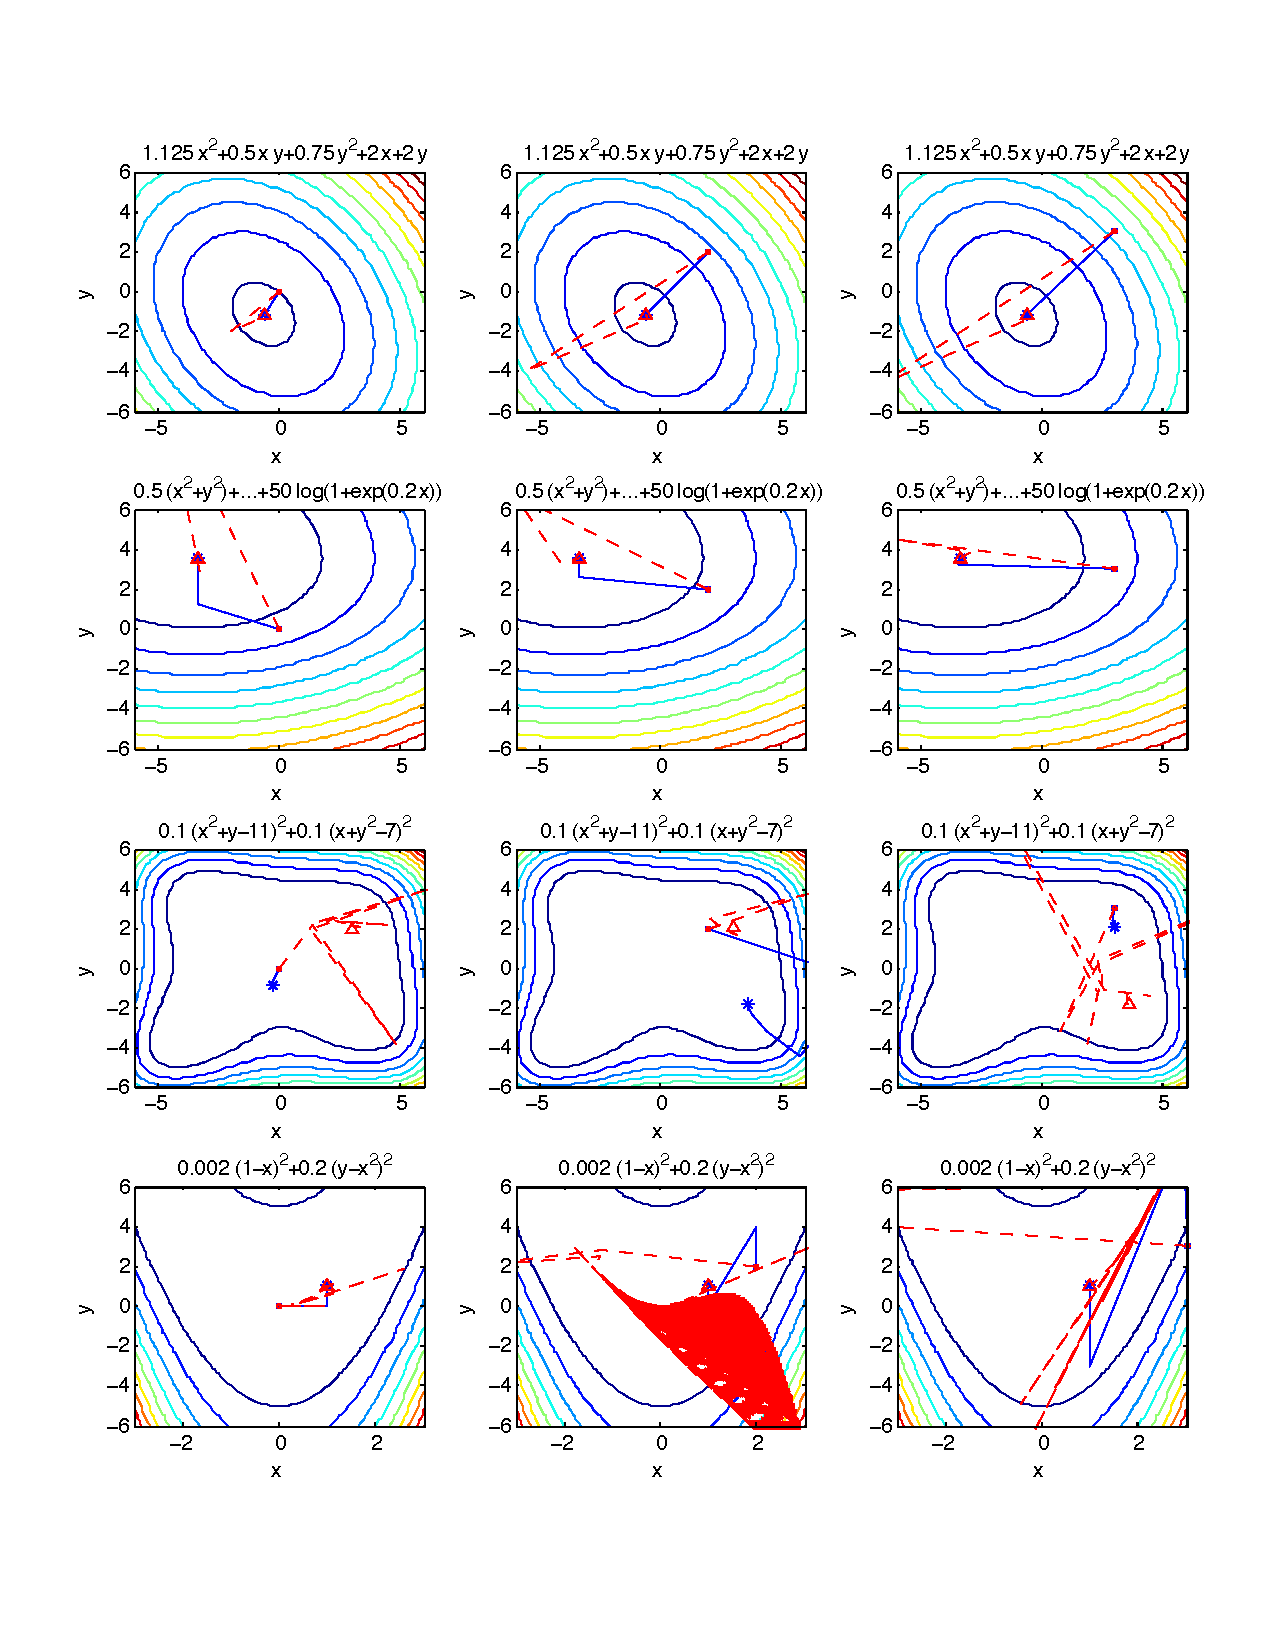
\includegraphics[width=0.7\textwidth]{img/p3Results.pdf}}
        \caption{Results for problem 3. We show each of the four functions (one
        per row), and the three initializations ($[0,0]$ in column 1, $[2,2]$
        in column 2, and $[3,3]$ in column 3). We plot both Newton's method
        (blue solid line) and BFGS (red dashed line) overlaid on the same
        axes.}
\end{figure}

(c) The final points gained from BFGS are sometimes different than those gained
via Newton's method. The two methods seem to converge to different solutions if
a method takes larger step sizes near the beginning of its progression that
takes it away from certain nearby local optima and into the range of another
local optima. The tracks for the other two initializations are shown in columns
2 and 3 of Figure 1. We see that, at times (namely, for the third function),
different initializations also produce different final points.

(d) In general, the number of iterations required for convergence via Newton's
method was the fewest, the number of iterations required for convergence via
BFGS was more (sometimes in the tens or hundreds), and the number of iterations
required for convergence via gradient descent was the most (often nearly
$20,000$ iterations required). There was one notable case, however, in the
fourth function, where BFGS became stuck in some sort of ``mode'', and took
over $4,000$ iterations before converging.

Given an arbitrary dimension $n$ (for the optimization variable), we can see
that the complexity of Newton's method is $O(n^3)$ (since it requires matrix
inversion), the complexity of BFGS is $O(n^2)$ (since it requires matrix-vector
multiplication), and the complexity of gradient descent is $O(n)$ (since this
is the complexity needed for computing each gradient).

\end{document}
